\chapter{Design Considerations}
\vspace{-5 mm}
In this chapter the system is designed with a top-down approach, which means an overview of the system is formulated first. Thereafter the system will be broken down into smaller segments.

First a use-case model of the system is given, where the functionalities and the coherent actors is described, in order to give an overview of what the system must be able to do. Thereafter, a description of provided vehicle and tracking system is made, to get a knowledge  base of the utilized systems. Constraints to the prototype will thereafter be set, caused by time limitations as well as a desired focus on the main scope of the project, in regards to the prototype, are considered.
\vspace{-4 mm}
\section{Use-case Design} \label{sec:UseCase}
To give an overview of what the system should be able to do, a use case with coherent actors is utilized. The use case diagram, see \figref{fig:usecase}, will describe the main functionalities in the use case as well as describing the actors, the external sensors and systems, affecting the system.

%The use-case diagram is made, where the micro controller is the system that will be analysed, because, it will be the master in this system
%
 \begin{figure}[H]
	\centering
	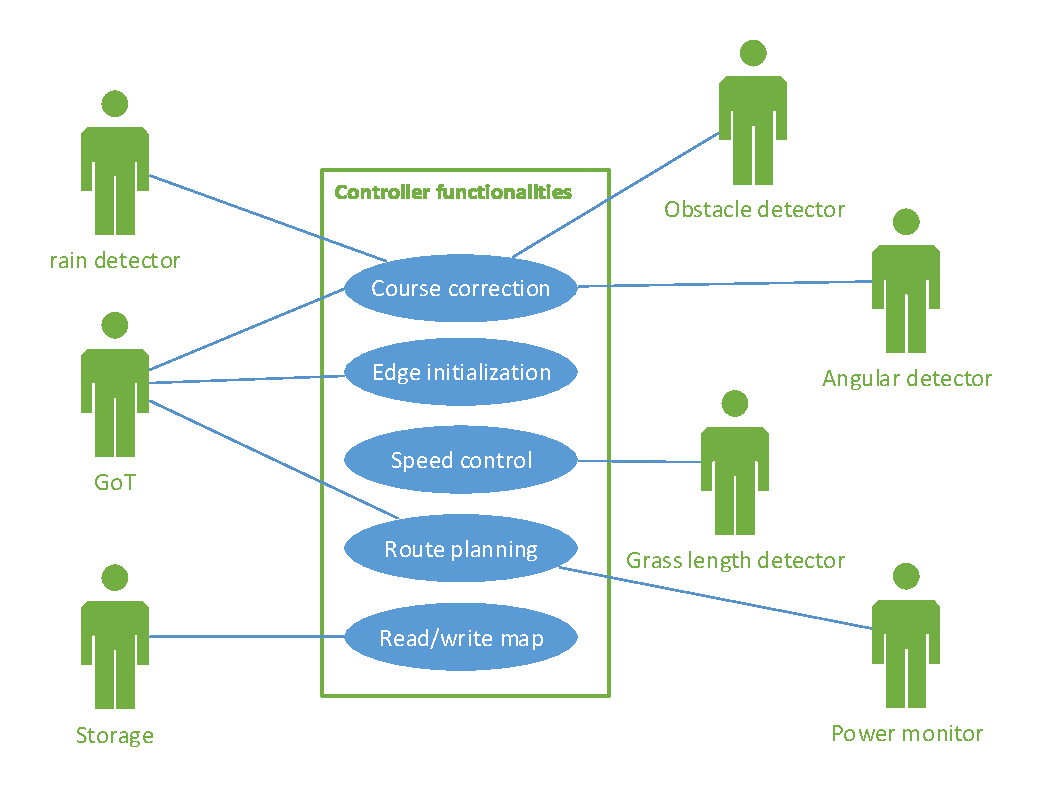
\includegraphics[scale=0.8]{figures/P5UseCase.pdf}
	\caption{Use-Case Diagram}
	\label{fig:usecase}
\end{figure}

\noindent
\newpage

The system, inside the controller, have 6 main functionalities and is affected by 9 different actors.

\subsection{Main Functionalities}

Functionalities are the functions that the system can do. Each functionality can have more than one function in the system. The functionalities get input from actors and can be in association with other functionalities. 

\textbf{Edge Initialization}:
The \textit{Edge Initialization} gets input from the \textit{GoT} system and is associated with the \textit{Read/Write Map} functionality. The purpose of this function, is to calibrate the system to a new lawn, by mapping the edge of the lawn. The edges which is mapped should include the area in which the vehicle should stay inside and the areas which it should avoid, e.g. trees, bushes and so on. This is done, by first manually moving the \textit{GoT} system's transmitter along the periphery of the lawn and thereafter along the edges of obstacle placed on the lawn. This could be performed by the use of a button which could make the system record edges if pressed. The information about the edges, an edge map is created and saved through the \textit{Read/Write Map} function.

\textbf{Route Planning}:
The \textit{Route Planning} gets input from the \textit{Power Monitor} and is associated with the \textit{Read/Write Map} functionality. The purpose of this function, is to plan the route for the lawn mower. The route is created by knowing where the lawn mower is located and the map of edges of the lawn, which is located in \textit{Storage}. The map is loaded from the \textit{Storage} with the \textit{Read/Write Map} function. Furthermore it acquires the voltage level of the battery from the \textit{Power Monitor}, to ensure it will return to base before it runs out of battery.

\textbf{Read/Write Map}:
The \textit{Read/Write Map} gets input from the \textit{Storage} and is associated with the \textit{Route Planning}, \textit{Course Correction} and the \textit{Edge Initialization} functionalities. This functionality is the link between functionalities and \textit{Storage}. The edge map retrieved from \textit{Edge Initialization} and through use of the \textit{Read/Write Map} function, is stored in the \textit{Storage}. In \textit{Storage}, the route which calculated by the \textit{Route Planning} is also located. The \textit{Course Correction} functionality also needs access to the \textit{Storage} to be able get the calculated route.

\textbf{Course Correction}:
The \textit{Course Correction} gets input from the \textit{GoT} system, the \textit{Humidity Detector}, the \textit{Obstacle Detector} and the \textit{Angular Detector} and is associated with the \textit{Read/Write Map} and the \textit{Speed Control} functionalities. This function gets both an angle and the humidity in the air as input, furthermore it gets an input if it encounters an obstacle blocking its path. \textit{Course Correction} takes all these parameters into consideration when navigating from its last registered position, retrieved from the \textit{GoT} system, to the next destination on the calculate route retrieved from the \textit{Storage} trough \textit{Read/Write Map}. The \textit{Course Correction} is the main function behind the regulation of the vehicle's angular movement, and therefore it can also regulate the vehicle back to the original path if it slips or is moved. The  \textit{Course Correction} decides the velocity, according to the calculated route, and passes the decided velocity to the \textit{Speed Control}.

\textbf{Speed Control}:
The \textit{Speed Control} gets input from  the \textit{Grass Length Detector} and the \textit{Speed Measurement} and is associated with \textit{Course Correction}. The function's purpose, is to make sure that the lawn mower adapts the speed depending on the grass length and if the \textit{Course Correction} ask for a different velocity, e.g. if the vehicle is going into a curve. additionally, if the \textit{Course Correction} ask for a desired velocity from the \textit{Speed Control}, it should be able to go to the desired velocity and maintain it regardless of incoming disturbances.

\textbf{Blade Control}:
The \textit{Blade Control} gets input from the \textit{Blade Monitor}. The function's purpose, is keeping the blade rotational speed the same, to make an even cut grass. With the input from the \textit{Blade Monitor}, the \textit{Blade Control} can regulate the velocity of the blade.

\subsection{Actors}
A actor is a component, that influence the system by giving inputs to the functionalities and/or receiving outputs from them.

\textbf{GoT}:
The \textit{GoT} system is connected to the \textit{Course Correction}, the \textit{Route Planning} and the \textit{Edge Initialization} functionalities. This system is used to retrieve the GoT transmitter's, placed on the vehicle, location on the lawn. The GoT system is explained in \secref{GoTDescription}.

\textbf{Storage}:
The \textit{Storage} is connected to the \textit{Read/Write Map} functionality. It uses a non-volatile storage to store the information about the edge map and route, which is made in the \textit{Edge Initialization} and \textit{Route Planning} functionalities. This will make the \textit{Storage} able to keep the data even if the system is turned off.

\textbf{Humidity Detector}:
The \textit{Humidity Detector} is connected to the functionality \textit{Course Correction}. This is a sensor that measures the humidity in the air. The system uses the information about the ambient humidity level to see, whether the grass is too wet for mowing the lawn, since wet grass can not be cut evenly. 

\textbf{Obstacle Detector}:
The \textit{Obstacle Detector} is connected to the \textit{Course Correction} functionality. This sensor detects, if there are any objects, which blocks the lawn mower's route. This sensor makes sure, that the lawn mower registers objects, like a human or a dog, which could interfere with the lawn mower's route.

\textbf{Angular Detector}:
The \textit{Angular Detector} is connected to the \textit{Course Correction} functionality. This sensor measures the angular position and movement of the lawn mower, whether it is intentional movement or if the lawn mower slips.

\textbf{Grass Length Detector}:
The \textit{Grass Length Detector} is connected to the \textit{Speed Control} functionality. This sensor measures the  grass length, which affects the velocity, at which the lawn mower should drive. If the grass is long, the lawn mower has to drive slower, to make sure that it cuts the grass evenly. 

\textbf{Power Monitor}:
The \textit{Power Monitor} is connected to the \textit{Route Planning} functionality. This sensor measures how much power is left in the battery. This is needed, so that the lawn mower can drive back to its charging station, before the battery is too low to make the vehicle run, and as well not damaging the battery.

\textbf{Blade Monitor}:
The \textit{Blade Monitor} is connected to the \textit{Blade Control} functionality. This sensor measures the rotational speed of the blade and send the information back to the \textit{Blade Control}

\textbf{Speed Measurement}:
The \textit{Speed Measurement} is connected to the \textit{Speed Control} functionality. The sensor measures the speed of the lawn mower.

These are some functionalities that could be implemented in a autonomous lawn mower. To get a knowledge base the provided vehicle and battery as well as the GoT system is described in the following section. 